\documentclass[journal, a4paper]{IEEEtran}

% some very useful LaTeX packages include:

%\usepackage{cite}      % Written by Donald Arseneau
                        % V1.6 and later of IEEEtran pre-defines the format
                        % of the cite.sty package \cite{} output to follow
                        % that of IEEE. Loading the cite package will
                        % result in citation numbers being automatically
                        % sorted and properly "ranged". i.e.,
                        % [1], [9], [2], [7], [5], [6]
                        % (without using cite.sty)
                        % will become:
                        % [1], [2], [5]--[7], [9] (using cite.sty)
                        % cite.sty's \cite will automatically add leading
                        % space, if needed. Use cite.sty's noadjust option
                        % (cite.sty V3.8 and later) if you want to turn this
                        % off. cite.sty is already installed on most LaTeX
                        % systems. The latest version can be obtained at:
                        % http://www.ctan.org/tex-archive/macros/latex/contrib/supported/cite/

\usepackage{graphicx}   % Written by David Carlisle and Sebastian Rahtz
                        % Required if you want graphics, photos, etc.
                        % graphicx.sty is already installed on most LaTeX
                        % systems. The latest version and documentation can
                        % be obtained at:
                        % http://www.ctan.org/tex-archive/macros/latex/required/graphics/
                        % Another good source of documentation is "Using
                        % Imported Graphics in LaTeX2e" by Keith Reckdahl
                        % which can be found as esplatex.ps and epslatex.pdf
                        % at: http://www.ctan.org/tex-archive/info/

%\usepackage{psfrag}    % Written by Craig Barratt, Michael C. Grant,
                        % and David Carlisle
                        % This package allows you to substitute LaTeX
                        % commands for text in imported EPS graphic files.
                        % In this way, LaTeX symbols can be placed into
                        % graphics that have been generated by other
                        % applications. You must use latex->dvips->ps2pdf
                        % workflow (not direct pdf output from pdflatex) if
                        % you wish to use this capability because it works
                        % via some PostScript tricks. Alternatively, the
                        % graphics could be processed as separate files via
                        % psfrag and dvips, then converted to PDF for
                        % inclusion in the main file which uses pdflatex.
                        % Docs are in "The PSfrag System" by Michael C. Grant
                        % and David Carlisle. There is also some information
                        % about using psfrag in "Using Imported Graphics in
                        % LaTeX2e" by Keith Reckdahl which documents the
                        % graphicx package (see above). The psfrag package
                        % and documentation can be obtained at:
                        % http://www.ctan.org/tex-archive/macros/latex/contrib/supported/psfrag/

%\usepackage{subfigure} % Written by Steven Douglas Cochran
                        % This package makes it easy to put subfigures
                        % in your figures. i.e., "figure 1a and 1b"
                        % Docs are in "Using Imported Graphics in LaTeX2e"
                        % by Keith Reckdahl which also documents the graphicx
                        % package (see above). subfigure.sty is already
                        % installed on most LaTeX systems. The latest version
                        % and documentation can be obtained at:
                        % http://www.ctan.org/tex-archive/macros/latex/contrib/supported/subfigure/

\usepackage{url}        % Written by Donald Arseneau
                        % Provides better support for handling and breaking
                        % URLs. url.sty is already installed on most LaTeX
                        % systems. The latest version can be obtained at:
                        % http://www.ctan.org/tex-archive/macros/latex/contrib/other/misc/
                        % Read the url.sty source comments for usage information.

%\usepackage{stfloats}  % Written by Sigitas Tolusis
                        % Gives LaTeX2e the ability to do double column
                        % floats at the bottom of the page as well as the top.
                        % (e.g., "\begin{figure*}[!b]" is not normally
                        % possible in LaTeX2e). This is an invasive package
                        % which rewrites many portions of the LaTeX2e output
                        % routines. It may not work with other packages that
                        % modify the LaTeX2e output routine and/or with other
                        % versions of LaTeX. The latest version and
                        % documentation can be obtained at:
                        % http://www.ctan.org/tex-archive/macros/latex/contrib/supported/sttools/
                        % Documentation is contained in the stfloats.sty
                        % comments as well as in the presfull.pdf file.
                        % Do not use the stfloats baselinefloat ability as
                        % IEEE does not allow \baselineskip to stretch.
                        % Authors submitting work to the IEEE should note
                        % that IEEE rarely uses double column equations and
                        % that authors should try to avoid such use.
                        % Do not be tempted to use the cuted.sty or
                        % midfloat.sty package (by the same author) as IEEE
                        % does not format its papers in such ways.

\usepackage{amsmath}    % From the American Mathematical Society
                        % A popular package that provides many helpful commands
                        % for dealing with mathematics. Note that the AMSmath
                        % package sets \interdisplaylinepenalty to 10000 thus
                        % preventing page breaks from occurring within multiline
                        % equations. Use:
%\interdisplaylinepenalty=2500
                        % after loading amsmath to restore such page breaks
                        % as IEEEtran.cls normally does. amsmath.sty is already
                        % installed on most LaTeX systems. The latest version
                        % and documentation can be obtained at:
                        % http://www.ctan.org/tex-archive/macros/latex/required/amslatex/math/



% Other popular packages for formatting tables and equations include:

%\usepackage{array}
% Frank Mittelbach's and David Carlisle's array.sty which improves the
% LaTeX2e array and tabular environments to provide better appearances and
% additional user controls. array.sty is already installed on most systems.
% The latest version and documentation can be obtained at:
% http://www.ctan.org/tex-archive/macros/latex/required/tools/

% V1.6 of IEEEtran contains the IEEEeqnarray family of commands that can
% be used to generate multiline equations as well as matrices, tables, etc.

% Also of notable interest:
% Scott Pakin's eqparbox package for creating (automatically sized) equal
% width boxes. Available:
% http://www.ctan.org/tex-archive/macros/latex/contrib/supported/eqparbox/

% *** Do not adjust lengths that control margins, column widths, etc. ***
% *** Do not use packages that alter fonts (such as pslatex).         ***
% There should be no need to do such things with IEEEtran.cls V1.6 and later.


% Your document starts here!
\begin{document}
\begin{titlepage}

\newcommand{\HRule}{\rule{\linewidth}{0.5mm}} % Defines a new command for the horizontal lines, change thickness here

\center % Center everything on the page
 %----------------------------------------------------------------------------------------
%	LOGO SECTION
%----------------------------------------------------------------------------------------

~\\[1cm]

\includegraphics{SCUT.png}\\[2cm] % Include a department/university logo - this will require the graphicx package

%----------------------------------------------------------------------------------------
%	TITLE SECTION
%----------------------------------------------------------------------------------------

\HRule \\[1cm]
{ \huge \bfseries The Experiment Report of \textit{Machine Learning} }\\[0.6cm] % Title of your document
\HRule \\[2cm]
%----------------------------------------------------------------------------------------
%	HEADING SECTIONS
%----------------------------------------------------------------------------------------


\textsc{\LARGE \textbf{School:} School of Software Engineering}\\[1cm]
\textsc{\LARGE \textbf{Subject:} Software Engineering}\\[2cm]


%----------------------------------------------------------------------------------------
%	AUTHOR SECTION
%----------------------------------------------------------------------------------------

\begin{minipage}{0.4\textwidth}
\begin{flushleft} \large
\emph{Author:}\\
Haipeng Deng % Your name
\end{flushleft}
\end{minipage}
~
\begin{minipage}{0.4\textwidth}
\begin{flushright} \large
\emph{Supervisor:} \\
Mingkui Tan% Supervisor's Name
\end{flushright}
\end{minipage}\\[2cm]
~
\begin{minipage}{0.4\textwidth}
\begin{flushleft} \large
\emph{Student ID:}\\
201730686193
\end{flushleft}
\end{minipage}
~
\begin{minipage}{0.4\textwidth}
\begin{flushright} \large
\emph{Grade:} \\
Undergraduate
\end{flushright}
\end{minipage}\\[2cm]

% If you don't want a supervisor, uncomment the two lines below and remove the section above
%\Large \emph{Author:}\\
%John \textsc{Smith}\\[3cm] % Your name

%----------------------------------------------------------------------------------------
%	DATE SECTION
%----------------------------------------------------------------------------------------

{\large \today}\\[2cm] % Date, change the \today to a set date if you want to be precise


%----------------------------------------------------------------------------------------

\vfill % Fill the rest of the page with whitespace

\end{titlepage}

% Define document title and author
	\title{Face Detection Based on AdaBoost Algorithm}
	\maketitle

% Write abstract here
\begin{abstract}
This report introduces my work in Lab3 : Face Detection Based on AdaBoost Algorithm in which I use some picture processing methods to make the raw material (training pictures data) suitable for fitting and first try Adaboost to implement a face classification model.
\end{abstract}

% Each section begins with a \section{title} command
\section{Introduction}
	% \PARstart{}{} creates a tall first letter for this first paragraph
\PARstart{T}{he} feature of the boosting algorithm is that there are strong dependencies between individual base learners and those learners are generated by the cascaded method. Adaboost (adaptive boosting) is one of the most famous boosting algorithms in ensemble learning. In this lab, I was required to implement a face classifying model using Adaboost. It was interesting to get familiar with the basic strategy of face detection and combine the theory I learned in class with this actual project practically for the first time. Besides, I was looking forward to experiencing the complete process of machine learning through this experiment.

% Main Part
\section{Methods and Theory}
In the practical classification problem, we will encounter some situation that one model can not separate the data of different labels well. To address this problem, a method called boosting is created. 
\begin{figure}[!hbt]
	% Center the figure.
	\begin{center}
	% Include the eps file, scale it such that it's width equals the column width. You can also put width=8cm for example...
	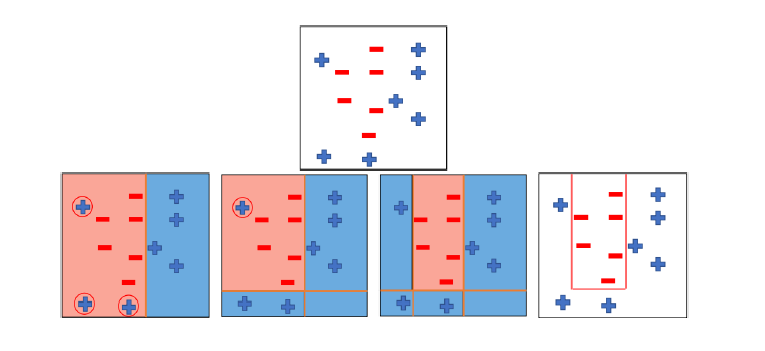
\includegraphics[width=\columnwidth]{intro_boosting.png}
	% Create a subtitle for the figure.
	\caption{Example using boosting algorithm}
	% Define the label of the figure. It's good to use 'fig:title', so you know that the label belongs to a figure.
	\label{fig1}
	\end{center}
\end{figure}\\
The Adaboost (adaptive boosting) model can be seen as a set of other models. In the training process, the boosting algorithm requires a base learner which trains on the original training set. Then it updates the weights of every single training datum according to the performance of this base learner i.e. enlarge the weight of those which is mistakenly classified to force the next learner focus it more and make the weight of correctly classified data smaller. In this lab it is implemented by the formula below:
\begin{align}
    w_{i+1} (i) = \frac{w_m(i)}{z_m} e^{-\alpha_my_ih_m(x_i)} \\
    z_m = \sum_{i=1}^n w_m(i) e^{-\alpha_my_ih_m(x_i)}
\end{align}\\
In order to evaluate the performance of every base learner we then introduce a term called error rate, which is computed as below:
\begin{equation}
    \epsilon_m = p(h_m(x_i) \neq y_i ) + \sum_{i=1}^n w_m(i)I(h_m(x_i) \neq y_i)
\end{equation}\\
In those base learner, we require that the performance of every one of them has the property $\epsilon_m < 0.5$.\\
So there comes another question, how should we determine the importance or weight for each base learner? To make the base learner with lower $\epsilon_m$ more important, an formula below gives us a solution:
\begin{equation}
    \alpha_m = \frac1 2 log(\frac{1-\epsilon_m}{\epsilon_m})
\end{equation}\\
By using the $\alpha_m$(s) computed above as the weights for base learners, we can finally assemble a final learner
\begin{equation}
    H(x) = sign(\sum_{m=1}^M \alpha_mh_m(x))
\end{equation}\\
Note: $h_m(x) = sign(w^Tx)$ is a nonlinear function, so the Adaboost can deal with nonlinear problem

\section{Experiments}
\subsection{Dataset}
The experiment document downloaded at Github provides 1000 pictures, of which 500 human face RGB images, stored in datasets/original/face; and 500 non-face RGB images, stored in datasets/original/nonface. In this lab, I do picture process and build my Adaboost model on the given dataset.

\subsection{Implementation}
\centering \textbf{Face Classification}\\
To start with, I load data set data and convert them into grayscale images with size of 24 * 24 and set the label of face images as $+1$ while the label of nonface images are $-1$.
% This is how you include a eps figure in your document. LaTeX only accepts EPS or TIFF files.
\begin{figure}[!hbt]
	% Center the figure.
	\begin{center}
	% Include the eps file, scale it such that it's width equals the column width. You can also put width=8cm for example...
	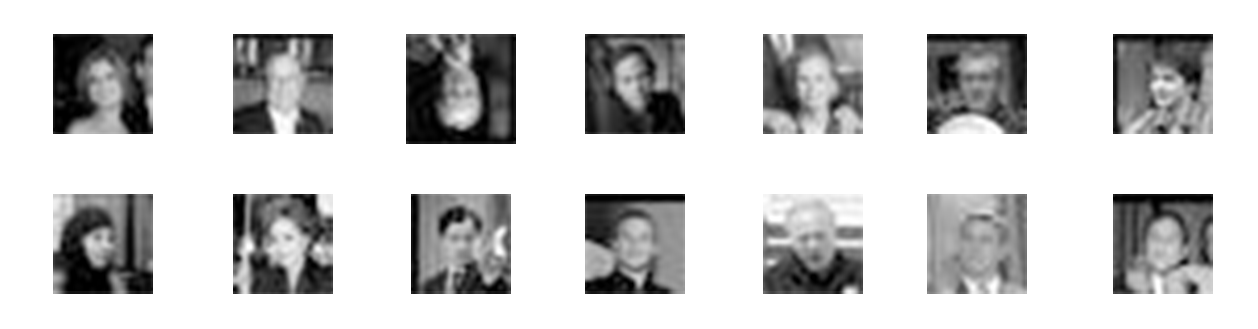
\includegraphics[width=\columnwidth]{photo_example.png}
	% Create a subtitle for the figure.
	\caption{Example of grey pictures}
	% Define the label of the figure. It's good to use 'fig:title', so you know that the label belongs to a figure.
	\label{fig2}
	\end{center}
\end{figure}\\
Secondly I use some already picture processing data code to extract NPD features of all pictures and store them in a numpy array. The following step I do is shuffling the data and splitting the dataset into a training set of 900 images and a validation set of 100 images. Then I implement all functions in AdaboostClassifier class which constructs an Adaboost model. In this part, I use 'DecisionTreeClassifier' in sklearn.tree library as my base learner class. Three base learners is assembled in my final classifier in total and their weight $\alpha$ is calculated using the formula mentioned above. Finally, the performance of my Adaboost model is shown below:
\begin{table}[!hbt]
	% Center the table
	\begin{center}
	% Title of the table
	\caption{Classifier Report}
	\label{tab:simParameters}
	% Table itself: here we have two columns which are centered and have lines to the left, right and in the middle: |c|c|
	\begin{tabular}{|c|c|c|c|c|}
		% To create a horizontal line, type \hline
		\hline
		% To end a column type &
		% For a linebreak type \\
		 & precision & recall & f1-score & support \\
		\hline
		$-1.0$ & $0.96$ & $0.96$ & $0.96$ & $51$\\
		\hline
		$1.0$ & $0.96$ & $0.96$ & $0.96$ & $49$\\
		\hline
		accuracy & & & $0.96$ & $100$\\
		\hline
        macro avg & $0.96$ & $0.96$ & $0.96$ & $100$\\
        \hline
        weighted avg & $0.96$ & $0.96$ & $0.96$ & $100$\\
        \hline
	\end{tabular}
	\end{center}
\end{table}\\

\centering \textbf{Face Detection}\\
In this part, I run $face detection.py$ and experience the OpenCV's built-in method of face detection using Haar Feature-based Cascade Classifiers.
\begin{figure}[!hbt]
	% Center the figure.
	\begin{center}
	% Include the eps file, scale it such that it's width equals the column width. You can also put width=8cm for example...
	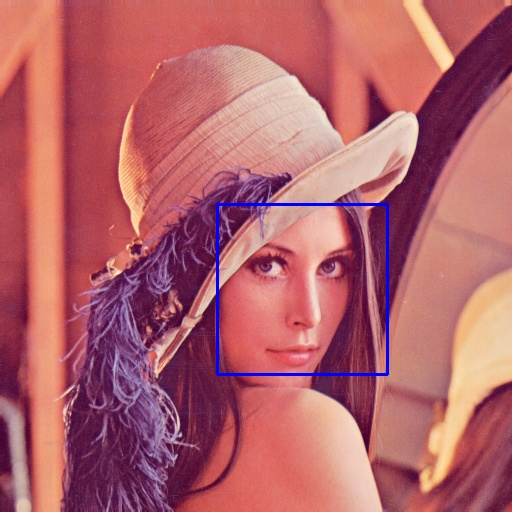
\includegraphics[width=\columnwidth]{result.jpg}
	% Create a subtitle for the figure.
	\caption{Result of OpenCV Face Detection}
	% Define the label of the figure. It's good to use 'fig:title', so you know that the label belongs to a figure.
	\label{fig2}
	\end{center}
\end{figure}\\
\par
	% If you have questions about how to write mathematical formulas in LaTeX, please read a LaTeX book or the 'Not So Short Introduction to LaTeX': tobi.oetiker.ch/lshort/lshort.pdf




\section{Conclusion}
	To summarize, I feel this lab very inspiring and beneficial for me. Instead of reading and deriving the theory and formulas in books and slices, it offers us a practical way to practise machine learning.



% Your document ends here!
\end{document}
